
\documentclass[11pt,letterpaper]{report}

% Paquetes
\usepackage[utf8]{inputenc}
\usepackage[spanish]{babel}
\usepackage[T1]{fontenc}
\usepackage[
    top=2.5cm,
    bottom=2.5cm,
    left=3.8cm,
    right=2.5cm
]{geometry}
\usepackage{graphicx}
\usepackage{url}
\usepackage{hyperref}
\usepackage{cite}
\usepackage[Sonny]{fncychap}
\usepackage{caption}
\usepackage{chngcntr}
\usepackage{float}

% Configuraciones iniciales
\bibliographystyle{IEEEtran}
\renewcommand{\citepunct}{],[}
\renewcommand{\citedash}{]--[}
\setlength{\parskip}{0.5\baselineskip}
\setlength{\parindent}{1.25cm}
\captionsetup[figure]{
    position=bottom,
    justification=centering,
    font=small,
    labelfont=normalfont
}
\counterwithout{figure}{chapter}
\captionsetup[table]{
    position=top,
    justification=centering,
    font=small,
    labelfont=normalfont
}
\counterwithout{table}{chapter}


\begin{document}

% Carátula
\begin{titlepage}
    \centering

    {\large UNIVERSIDAD DEL VALLE DE GUATEMALA\par}
    \vspace{0.3cm}
    {\large Facultad de Ingeniería\par}

    \vfill

    
\includegraphics[width=0.65\textwidth]{imagenes/logoHD}

    \vfill

    {\bfseries\large IMPLEMENTACIÓN DE UN SISTEMA ADAPTATIVO DE INTERACCIÓN
    Y AJUSTE DE DIFICULTAD DINÁMICO PARA UNA EXPERIENCIA DE VIDEOCLIP
    GAMIFICADO EN REALIDAD VIRTUAL\par}

    \vfill

    {\large Diego García, 22404\par}

    \vfill

    {\large Ingeniería en Ciencias de la Computación y Tecnología de la Información\par}
    \vspace{0.3cm}
    {\large Trabajo Profesional\par}
    \vspace{0.3cm}
    {\large Guatemala, 2026\par}

\end{titlepage}

% Páginas preliminares
\pagenumbering{roman}
\setcounter{page}{1}

% Indice
\tableofcontents


% Resumen
\clearpage
\newgeometry{
    top=5cm,
    bottom=2.5cm,
    left=3.8cm,
    right=2.5cm
}
\chapter*{Resumen}
\phantomsection
\addcontentsline{toc}{chapter}{Resumen}
El presente proyecto propone la implementación de un sistema de 
interacción adaptativa en realidad virtual (VR, por sus siglas 
en inglés) para una experiencia de videoclip gamificado. Su 
enfoque es el desarrollo de un mecanismo capaz de registrar 
métricas de desempeño del usuario en tiempo real, interpretar 
estados de interacción y ajustar dinámicamente parámetros del 
\textit{gameplay}, como la velocidad, cantidad de objetos y complejidad 
de las tareas. Esto, basándose en el diseño de interfaces de 
interacción en VR, técnicas de interacción en entornos 
inmersivos, adaptación basada en experiencia del jugador, 
retroalimentación multisensorial y evaluación de presencia 
y experiencia de usuario.

Para el desarrollo del sistema se utiliza Unity para la lógica 
interactiva y el prototipado de la experiencia, mientras que los 
modelos en 3D se crean en Blender. El desarrollo conlleva un 
prototipo funcional que integre entrada de VR, detección de 
interacción, almacenamiento de métricas en tiempo real, lógica de 
estados del jugador y adaptación dinámica. Como resultado, se 
busca aportar una base técnica y metodológica para experiencias 
inmersivas que no solo respondan a las entradas del usuario, sino
también ajusten su comportamiento en función del desempeño y de 
indicadores de involucramiento durante la experiencia.

\clearpage
\restoregeometry

% Capítulos
\pagenumbering{arabic}
\setcounter{page}{1}

% Introducción
\chapter{Introducción}

La realidad virtual (VR, por sus siglas en inglés) se ha 
consolidado como un campo de investigación relevante dentro del 
desarrollo de experiencias digitales inmersivas, sobre todo en lo
relacionado con el diseño de interfaces, técnicas de interacción
y evaluación de la experiencia de 
usuario \cite{chen2024interfaces}. Estudios recientes muestran 
que la interacción en entornos virtuales no puede abordarse 
únicamente desde una perspectiva técnica, sino que requiere 
considerar criterios de usabilidad, naturalidad, 
retroalimentación y un contexto adecuado para la experiencia 
\cite{chen2024interfaces,spittle2023interaction,yeo2024interfaces}. Con eso 
en mente, este proyecto propone la implementación de un sistema de 
interacción adaptativa en VR para una experiencia de videoclip gamificado. 
La propuesta se enfoca en el desarrollo de una solución capaz de registrar 
métricas de desempeño del usuario en tiempo real, interpretar estados de 
interacción y ajustar dinámicamente parámetros del \textit{gameplay}, con el
fin de construir una experiencia más sensible al comportamiento del jugador 
y una mejor integridad al flujo general de la aplicación.

El valor de este proyecto se sustenta en investigaciones recientes sobre 
adaptación en videojuegos y entornos interactivos han señalado que, aunque 
existen avances importantes en personalización, modelado del jugador y 
ajuste dinámico del contenido, aún queda una brecha en la integración 
completa del ciclo conformado por las sensaciones del usuario, la 
interpretación de su estado y la modificación adaptativa de la experiencia 
en tiempo real \cite{lopes2025closing}. Debido a esto, resulta académica y
técnicamente relevante desarrollar prototipos que articulen la telemetría 
del usuario con mecanismos de adaptación concretos dentro de experiencias 
inmersivas. A su vez, investigaciones sobre ajustes dinámicos de dificultad 
en VR evidencian que la adaptación puede ir más allá de simples cambios de 
nivel, permitiendo modificar velocidad, complejidad y estructura de las 
tareas de acuerdo con las capacidades o desempeño del usuario 
\cite{huber2021dda}. Esto resulta particularmente valioso en una experiencia 
de videoclip gamificado, donde el equilibrio entre reto, ritmo, claridad e
involucramiento constituye un factor central para sostener la atención del 
jugador y favorecer una participación más fluida.

De igual manera, dentro de la industria, la relevancia que adquiere el 
proyecto se relaciona con la creciente necesidad de diseñar experiencias 
inmersivas que no sean estáticas, sino capaces de responder al usuario de 
manera contextual \cite{lopes2025closing,huber2021dda}. La revisión 
sistemática de Lopes et al. señala que los sistemas adaptativos orientados 
por la experiencia del jugador representan una dirección prometedora para 
incrementar la personalización y la inmersión en aplicaciones interactivas
\cite{lopes2025closing}. Las investigaciones sobre evaluación en VR también 
reportan que constructos como presencia, experiencia de usuario y mareos 
virtuales constituyen dimensiones centrales para valorar la calidad de una 
experiencia inmersiva, y que su análisis suele beneficiarse de la 
combinación entre métricas objetivas y herramientas subjetivas de 
evaluación \cite{wang2025presence,bareisyte2024questionnaires}. De la misma 
manera, se ha documentado que el \textit{feedback} visual y háptico puede contribuir 
positivamente a la sensación de presencia, mientras que la carga de tareas 
y las exigencias impuestas al usuario pueden influir en el nivel de malestar 
o mareos virtuales \cite{sepich2022workload,gibbs2022feedback}. Por ello, 
el proyecto no solo resulta importante por su componente técnico, sino 
también por su potencial para explorar cómo la adaptación dinámica puede 
incidir en la calidad de la experiencia inmersiva.

Como antecedentes, se han desarrollado diferentes propuestas que demuestran 
la viabilidad de utilizar información observable del jugador para modificar 
una experiencia interactiva durante su ejecución. Algunos sistemas han 
construido modelos a partir del comportamiento registrado durante la partida
para seleccionar modificaciones orientadas a mejorar la experiencia estimada
del usuario \cite{yannakakis2009adaptation}. Otros trabajos han considerado 
la dificultad como un fenómeno temporal, analizando tendencias a lo largo de
varias interacciones antes de decidir si el desafío debe incrementarse, 
mantenerse o reducirse \cite{zook2012temporal,xue2017dda}. Dentro del contexto específico de VR, también se han implementado mecanismos de ajuste
dinámico capaces de modificar la estructura y complejidad de las tareas de acuerdo con
información obtenida del usuario \cite{huber2021dda}. Estas aproximaciones 
evidencian que el desempeño del jugador puede utilizarse como una variable 
dinámica y no únicamente como un resultado evaluado al finalizar una sesión. 
También muestran que la adaptación en VR puede intervenir directamente sobre 
variables del \textit{gameplay} y no limitarse a niveles generales de 
dificultad. Paralelamente, los videojuegos musicales han desarrollado 
distintas formas de integrar la música con las acciones del jugador, 
utilizando elementos sonoros y temporales como parte de las propias reglas 
de interacción \cite{pichlmair2007sound}. Sin embargo, la integración 
conjunta de una experiencia musical en VR con un sistema que registre y 
modifique parámetros del \textit{gameplay} en tiempo real representa una 
convergencia menos desarrollada.

El proyecto se desarrolla en un lapso de cinco meses y está orientado a la 
construcción de un prototipo académico funcional en Unity, utilizando 
Blender para la creación de algunos recursos tridimensionales. El desarrollo
se enfoca en la interacción base en VR, el registro de métricas de desempeño, 
el modelado de estados de interacción y la adaptación dinámica del gameplay.
Para ello, se consideran las siguientes métricas: errores, tiempo de 
reacción, precisión y frecuencia de interacción. Estas métricas permiten 
observar tendencias en el comportamiento del jugador durante la ejecución de
la experiencia. A partir de ellas, el sistema utilizará estados discretos como 
representaciones computacionales del comportamiento observado y podrá 
modificar parámetros directamente relacionados con el \textit{gameplay}, 
principalmente velocidad, cantidad de objetos y complejidad de las tareas. 
Estos estados no pretenden construir diagnósticos psicológicos o clínicos, 
sino abstracciones operativas orientadas a la toma de decisiones dentro del 
sistema adaptativo.

El alcance contempla también los mecanismos necesarios para producir y 
registrar dichas interacciones, entre ellos entrada mediante controles, 
detección de colisiones, reglas de juego y retroalimentación visual y háptica. 
Por otra parte, quedan fuera del desarrollo los componentes relacionados con
la secuenciación temporal global del videoclip, la administración general
del tiempo de la canción, la activación global de escenas, la sincronización
audiovisual general y la persistencia del progreso. Estos elementos podrán 
comunicarse con el sistema adaptativo, pero no forman parte del mecanismo de 
medición, modelado y ajuste desarrollado en este trabajo. Asimismo, se 
excluyen la comercialización del producto final y cualquier validación 
clínica de estados cognitivos complejos.

Las pruebas realizadas con 34 participantes generan 5048 registros de 
interacción distribuidos entre los seis minijuegos de la experiencia y 
muestran que el sistema es capaz de registrar diferencias de desempeño, 
representar cambios mediante estados operativos y modificar la 
dificultad durante la ejecución. El sistema de adapatación dinámica de 
dificultad (DDA, por sus siglas en inglés) realiza 216 cambios de 
dificultad y, entre los ajustes que permiten comparar cinco 
interacciones antes y después, las reducciones presentan un aumento 
promedio en la tasa de éxito de 34.71\% a 62.06\%, mientras que los 
aumentos de dificultad producen una reducción de 91.30\% a 60.00\%, 
evidenciando un cambio observable en la exigencia de las actividades. 
En la evaluación subjetiva, el 67.65\% de los participantes reporta 
niveles altos de atención a la canción, el 96.97\% de las respuestas 
válidas califica la diversión con valores de 4 o 5 y el 73.53\% indica 
sentirse nada o ligeramente abrumado. Estos resultados respaldan el 
funcionamiento del sistema de interacción adaptativa, aunque no permiten 
atribuir directamente las valoraciones subjetivas al DDA.



% Objetivos
\chapter{Objetivos}

\section{Objetivo general}
\label{sec:objetivoGeneral}
Implementar un sistema de interacción adaptativa en realidad virtual (VR, 
por sus siglas en inglés) para un videoclip gamificado, capaz de registrar 
métricas del usuario, modelar estados de interacción y ajustar dinámicamente
parámetros del juego en tiempo real.

\section{Objetivos específicos}
\label{sec:objetivosEspecificos}
\begin{enumerate}
    \item Desarrollar en Unity el sistema base de interacción en VR, 
    incluyendo entrada mediante controladores o manos, detección de 
    colisiones, reglas de juego y mecanismos de retroalimentación visual y 
    háptica.

    \item Implementar un mecanismo de captura y almacenamiento de métricas 
    que registre aciertos, errores y frecuencia de interacción durante el
    \textit{gameplay}, para apoyar el análisis del comportamiento del usuario.

    \item Integrar un sistema de adaptación dinámica que modifique los 
    parámetros de velocidad, cantidad de objetos y complejidad de la 
    experiencia.
\end{enumerate}

% Justificación
\chapter{Justificación}

El desarrollo de experiencias inmersivas en realidad virtual (VR, 
por sus siglas en inglés) ha evolucionado desde esquemas 
centrados únicamente en la interacción básica hacia enfoques que
consideran el comportamiento del usuario como componente para 
modificar la experiencia en tiempo real \cite{lopes2025closing}. 
Estudios recientes muestran que el diseño de interfaces de 
interacción en VR, las técnicas de interacción en entornos 
inmersivos y las interfaces tridimensionales constituyen áreas
activas de investigación, debido a que la calidad de la 
experiencia depende no solo de la representación visual del 
entorno, sino también de la forma en la que el usuario interactúa 
con él \cite{chen2024interfaces,yeo2024interfaces}. Bajo este 
enfoque, es importante plantear la creación de una experiencia 
que no se limite a implementar mecánicas interactivas, sino que 
incorpore una capa adaptativa capaz de responder al 
comportamiento del jugador.

La relevancia de este proyecto se encuentra en la necesidad de 
avanzar hacia experiencias interactivas más sensibles a las 
características y respuestas de cada usuario. La literatura sobre
adaptación basada en la experiencia del jugador ha identificado 
que aún persiste una brecha entre la captura de información del 
usuario, la interpretación de su estado y la aplicación de 
cambios efectivos en tiempo real del sistema \cite{lopes2025closing}.
Esto es significativo porque la personalización no depende únicamente 
de observar métricas, sino de convertirlas en decisiones capaces de 
ajustar la experiencia de manera coherente con las necesidades del 
jugador. En este sentido, una experiencia musical interactiva representa 
un escenario particularmente valioso, ya que en ella no solo importa el 
cumplimiento de objetivos o tareas, sino también la conservación de un 
equilibrio entre reto, inmersión y apreciación de la música y del 
entorno \cite{pichlmair2007sound}. Precisamente por esa necesidad de 
balance, este tipo de propuesta ofrece un contexto adecuado para 
examinar el potencial de la adaptación dinámica como medio para 
enriquecer la experiencia del usuario.

Desde el punto de vista técnico, la adaptación dinámica puede 
construirse a partir de variables observables del comportamiento del 
jugador. En particular, se ha reportado que sistemas de ajuste dinámico 
de dificultad pueden modificar parámetros del juego en tiempo real con 
base en el desempeño del usuario, por ejemplo, mediante cambios en 
velocidad, complejidad o estructura de las tareas \cite{huber2021dda}.
De igual forma, revisiones recientes sobre estimación de 
\textit{engagement} en videojuegos indican que las métricas utilizadas 
con mayor frecuencia para modelar el estado del jugador incluyen señales 
de desempeño, patrones de interacción, telemetría del juego y, en ciertos 
casos, información fisiológica, lo que confirma que la captura de 
métricas en \textit{runtime} constituyen una base válida para construir 
mecanismos de adaptación \cite{rashed2025engagement}.

La implementación de adaptación dinámica también presenta dificultades 
que justifican la necesidad de diseñar cuidadosamente la relación entre 
métricas y modificaciones del \textit{gameplay} 
\cite{xue2017dda,zohaib2018dda}. Un sistema excesivamente sensible puede 
responder a variaciones aisladas del desempeño y producir cambios 
frecuentes o contradictorios en la dificultad. De igual forma, 
modificaciones demasiado evidentes pueden afectar la percepción de 
control del jugador o alterar la comprensión de las reglas de la 
experiencia \cite{lopes2025closing,zook2012temporal}. Por ello, la
adaptación no consiste únicamente en detectar un error y disminuir 
inmediatamente la dificultad, sino en interpretar tendencias 
suficientemente estables antes de modificar las condiciones del juego.

Además de controlar cuándo y con qué frecuencia se realizan los ajustes, 
debe considerarse que un buen desempeño no representa necesariamente una 
experiencia satisfactoria, así como la presencia de errores no implica 
por sí misma una experiencia negativa \cite{yannakakis2009adaptation,rashed2025engagement}.
Esta consideración adquiere mayor importancia en VR, donde constructos 
como presencia, experiencia de usuario y \textit{cybersickness} son 
dimensiones centrales para valorar la calidad de una aplicación 
inmersiva \cite{wang2025presence,bareisyte2024questionnaires}. 
Incrementar factores como la velocidad, cantidad de objetos o la 
complejidad puede elevar simultáneamente las exigencias de la 
actividad \cite{sepich2022workload}. El análisis de estos constructos se 
beneficia de la combinación entre métricas objetivas y herramientas 
subjetivas de evaluación. También se ha observado que el 
\textit{feedback} visual y háptico puede incrementar la sensación de 
presencia, mientras que la carga de tarea puede influir en mareos y otros 
malestares \cite{sepich2022workload,gibbs2022feedback}. Por ello, resulta 
relevante diseñar un sistema que utilice varias métricas de interacción 
y reglas de adaptación controladas, procurando conservar un equilibrio 
entre desafío, claridad, \textit{confort} e involucramiento en lugar de 
optimizar únicamente la cantidad de aciertos del usuario.

Otro valor que tiene este proyecto radica en la necesidad de estudiar 
las experiencias inmersivas desde una perspectiva más integral, ya que 
diversos componentes que influyen en la calidad de la interacción, como 
la retroalimentación multisensorial, el comportamiento del usuario y la 
adaptación del sistema, suelen analizarse de manera aislada \cite{chen2024interfaces,spittle2023interaction,yeo2024interfaces,lopes2025closing,huber2021dda}.
Esta separación limita la comprensión de cómo dichos elementos se 
relacionan entre sí dentro de una experiencia real de uso. En 
consecuencia, resulta pertinente desarrollar propuestas que permitan 
observar de forma conjunta cómo la interacción, las métricas del 
usuario y la adaptación dinámica pueden incidir en la personalización y 
en la capacidad de respuesta del sistema frente al contexto de uso \cite{lopes2025closing,rashed2025engagement}.
Visto así, el proyecto adquiere valor tanto para la investigación como 
para la industria, al aportar un caso aplicado que puede contribuir a 
la comprensión de cómo diseñar experiencias gamificadas más sensibles 
al usuario y mejor fundamentadas en datos de interacción.

% Marco teórico
\chapter{Marco Teórico}

\section{Realidad Virtual e interacción inmersiva}
La investigación sobre la realidad virtual (VR, 
por sus siglas en inglés) ha evolucionado más 
allá de solo buscar una experiencia tridimensional 
hacia la integración en las interacciones y la 
experiencia del usuario. Las aplicaciones 
inmersivas actuales no dependen únicamente de la 
calidad gráfica del entorno, sino también de la 
correspondencia entre las acciones físicas 
realizadas por el usuario, las respuestas 
producidas por el sistema y los mecanismos 
mediante los cuales se comunican los resultados 
de cada interacción \cite{chen2024interfaces,spittle2023interaction,yeo2024interfaces}.
Como consecuencia, el diseño de experiencias de 
VR abarca un campo interdisciplinario en el que 
se unen aspectos computacionales, perceptuales y 
ergonómicos.

Las interfaces de interacción en VR ocupan 
diferentes mecanismos de entrada, seguimiento y 
retroalimentación, entre ellos controladores, 
seguimiento de manos, reconocimiento de gestos y 
dispositivos hápticos \cite{chen2024interfaces}. 
Por ello, la incorporación de una tecnología de 
entrada no garantiza por sí sola una interacción 
adecuada, sino que debe responder a las tareas 
que forman parte de la experiencia. Las técnicas 
de interacción empleadas en entornos inmersivos 
pueden organizarse de acuerdo con tareas como la 
selección, la manipulación, la navegación y el 
control del sistema \cite{spittle2023interaction}.
No existe una técnica de interacción que resulte 
igualmente efectiva para todas las aplicaciones, 
pues su utilidad depende de las características 
de los objetos, la actividad realizada, el 
\textit{hardware} disponible y el contexto de uso. 
Esta dependencia del contexto es especialmente 
relevante en experiencias gamificadas, donde una 
misma sesión puede incluir acciones diferentes 
como apuntar, alcanzar, desplazarse o activar 
elementos virtuales.

Durante las primeras investigaciones sobre 
interfaces tridimensionales también se demostró 
que una interacción técnicamente funcional no 
necesariamente produce una experiencia 
comprensible o satisfactoria \cite{yeo2024interfaces}.
Las técnicas de selección y manipulación deben 
proporcionar señales que permitan reconocer qué 
objetos pueden utilizarse, cuando se ha detectado 
una acción y cuál ha sido su resultado \cite{chen2024interfaces}.
En consecuencia, la claridad de una interacción 
depende tanto de la entrada ejecutada por el 
usuario como de la respuesta inmediata que el 
sistema genera.

La retroalimentación visual y háptica ha sido 
investigada como un medio para comunicar el 
estado de los objetos y confirmar el resultado de 
las acciones dentro de entornos virtuales \cite{chen2024interfaces,gibbs2022feedback}.
La combinación de diferentes canales sensoriales puede contribuir a que 
el usuario perciba una relación más clara entre sus movimientos físicos 
y los acontecimientos del entorno virtual. La retroalimentación 
multisensorial no debe considerarse únicamente como un componente 
estético, sino como una parte funcional de la interfaz que permite 
informar sobre aciertos, errores, contacto con objetos y cambios en el 
estado del sistema.

Además de la interacción, también se ha estudiado dimensiones como la 
presencia, la experiencia de usuario y el \textit{cybersickness}. Estos 
elementos permiten examinar la calidad de una experiencia inmersiva más 
allá de su funcionamiento técnico \cite{wang2025presence,bareisyte2024questionnaires}.
La presencia se relaciona con la percepción de encontrarse dentro del 
entorno virtual, mientras que el \textit{cybersickness} trata de 
diferentes formas de malestar que pueden surgir durante el uso de 
dispositivos VR \cite{sepich2022workload}. Debido a que ambas 
dimensiones pueden estar influenciadas por el diseño de las tareas, la 
retroalimentación y la carga impuesta al usuario, resultan relevantes al 
analizar aplicaciones interactivas en VR \cite{gibbs2022feedback}.

La evaluación de experiencias de VR suele combinar información objetiva 
registrada por el sistema con información subjetiva proporcionada por 
los participantes \cite{wang2025presence,bareisyte2024questionnaires}.
Las métricas fisiológicas y conductuales pueden utilizarse para 
complementar la medición de presencia, aunque su interpretación depende 
del contexto y de las condiciones específicas de cada experiencia. De 
manera similar, existe una amplia variedad de cuestionarios orientados a 
evaluar presencia, usabilidad, experiencia de usuario y malestar, pero 
no todos utilizan las mismas definiciones ni miden exactamente los 
mismos componentes. Por esta razón, la selección de instrumentos y 
métricas debe responder a los objeticos concretos de cada investigación.

La carga generada por una tarea puede influir en el nivel de malestar 
experimentado por el usuario dentro de un entorno virtual \cite{sepich2022workload}.
Esto implica que la dificultad de una actividad inmersiva no debe 
evaluarse únicamente mediante tasas de éxito o fracaso. Una tarea 
excesivamente rápida, compleja o demandante también puede afectar la 
claridad de la interacción y el \textit{confort} del participante. La 
adaptación dentro de una aplicación inmersiva no puede plantearse 
únicamente como un mecanismo para aumentar o disminuir la dificultad, 
sino como una herramienta para mantener condiciones de interacción 
apropiadas para el comportamiento observado del usuario. Por ello, un 
sistemas adaptativos, debe modificar la dificultad tomando en cuenta 
como eso altera las exigencias que la experiencia impone al usuario.

\section{Videojuegos y experiencias musicales interactivas}
La relación entre música e interacción de videojuegos ha sido estudiada 
desde distintas formas de participación del jugador y de integración del 
sonido con las mecánicas. En particular, la literatura sobre 
interactividad en videojuegos musicales identifica principios mediante 
los cuales la música puede incorporarse a las reglas, acciones, 
estructuras temporales y mecanismos de respuesta de una experiencia 
interactiva \cite{pichlmair2007sound}. A partir de este enfoque, los 
videojuegos musicales pueden analizarse no únicamente por utilizar 
música como acompañamiento, sino por la forma en que los elementos 
musicales intervienen directamente en el \textit{gameplay}.

Existen múltiples maneras en las que se puede interactuar en un 
videojuego musical, como la ejecución de acciones rítmicas, el 
seguimiento de una estructura temporal, la asociación entre sonido y 
elementos visuales, la interpretación de secuencias y la modificación de 
componentes sonoros \cite{pichlmair2007sound}. Estas formas de interacción crean diferentes niveles 
de participación. En algunos casos, el usuario crea o modifica 
directamente el sonido, mientras que en otros ejecuta acciones que son 
evaluadas de acuerdo con que tanto se apeguen a una estructura musical 
establecida. 

La música también puede cumplir varias funciones dentro de una 
experiencia interactiva. Puede actuar como guía temporal, como 
respuesta a las acciones realizadas, como elemento que organiza la 
progresión o como parte central de las reglas del juego. Esto diferencia 
a las experiencias musicales interactivas de aquellas en las que una 
canción funciona únicamente como fondo sonoro. En una experiencia 
gamificada, la relación entre música y acción puede determinar cuándo 
debe intervenir el usuario, qué tipo de respuesta debe realizar y cómo 
se comunica el resultado de su participación \cite{rashed2025engagement}.

Lo anterior crea un reto para el desarrollador. Las exigencias del 
\textit{gameplay} deben permitir que el usuario participe activamente 
sin desplazar por completo su atención de la música y del entorno. 
Cuando las tareas requieren una concentración excesiva o presentan una 
dificultad inadecuada, la experiencia puede convertirse únicamente en 
una cadena de objetivos mecánicos \cite{rashed2025engagement}. Por el 
contrario, una actividad con muy poca exigencia puede reducir el 
involucramiento del jugador. La literatura sobre videojuegos musicales 
plantea, por tanto, la necesidad de conservar una relación coherente 
entre sonido, interacción, dificultad y respuesta del sistema.

\section{Adaptación dinámica y ajuste de dificultad}
La adaptación dinámica en videojuegos comprende enfoques en los que la 
información obtenida durante la interacción del jugador se utiliza para 
modificar distintos componentes de la experiencia. Las revisiones sobre 
adaptación basada en la experiencia describen este proceso como un ciclo 
en el que se observa al usuario, se interpreta su comportamiento y, 
posteriormente, se aplican cambios sobre elementos controlables del 
juego \cite{lopes2025closing}. Desde esta perspectiva, la adaptación 
busca reducir rigidez de experiencias que mantienen las mismas 
condiciones para todos los jugadores, permitiendo que el sistema 
responda a diferencias de desempeño y a cambios que ocurren durante una 
misma sesión.

Para completar este ciclo, la recopilación de información por sí sola no 
es suficiente. Las métricas registradas deben convertirse en una 
representación útil del jugador y, después, en decisiones capaces de 
modificar elementos concretos de la experiencia. La conexión entre 
medición, interpretación y modificación constituye uno de los aspectos 
centrales del diseño de sistemas adaptativos. En una experiencia musical 
interactiva, esta relación adquiere especial importancia porque los 
cambios deben responder al desempeño sin romper la coherencia entre 
\textit{gameplay}, interacción y experiencia musical \cite{pichlmair2007sound}.

Una de las formas más documentadas de adaptación es el ajuste dinámico 
de dificultad (DDA, por sus siglas en inglés). Este método modifica 
automáticamente características, comportamientos o escenarios de un 
videojuego durante su ejecución a partir de la habilidad o del desempeño 
observado en el jugador \cite{zohaib2018dda}. A diferencia de los niveles 
seleccionados antes de comenzar una partida, el ajuste dinámico puede 
responder a cambios ocurridos durante una misma sesión.

Los sistemas DDA pueden modificar parámetros como la velocidad, la 
cantidad de elementos, la disponibilidad de recursos, el comportamiento 
de los oponentes, la frecuencia de aparición de objetos y la complejidad 
de las tareas \cite{zohaib2018dda,huber2021dda}. En VR, también se ha 
investigado la generación y modificación de contenido con base en la 
experiencia del usuario, demostrando que la adaptación puede intervenir 
sobre la estructura de una actividad y no únicamente cambiar una 
etiqueta general de dificultad. La implementación de estos sistemas 
puede apoyarse en reglas heurísticas, modelos probabilísticos, 
redes neuronales, algoritmos evolutivos y otras técnicas de inteligencia 
computacional. No obstante, la utilización de modelos complejos no es un 
requisito para una solución adaptativa. Cuando el conjunto de métricas y 
parámetros está claramente delimitado, un sistema basado en reglas puede 
ofrecer cambios comprensibles, controlables y verificables durante el 
desarrollo. Un sistema adaptativo suele requerir un mecanismo que 
observe al jugador, una representación de su situación y un 
procedimiento que seleccione cambios en el videojuego. La observación 
puede realizarse mediante telemetría producida durante la partida. La 
representación puede consistir en valores numéricos, categorías o 
estados. Finalmente, el mecanismo de decisión determina qué parámetro 
debe modificarse, en qué magnitud y durante cuánto tiempo.

Los modelos temporales de jugador han demostrado que el desempeño no 
debe tratarse necesariamente como una característica estática \cite{zook2012temporal}.
Las capacidades observadas pueden cambiar conforme el usuario aprende 
las reglas, se acostumbra a los controles o enfrenta nuevas tareas. Por 
ello, un sistema de adaptación puede beneficiarse de analizar secuencias 
de interacciones y tendencias de desempeño, en lugar de reaccionar de 
manera inmediata ante cada acierto o error aislado.

La adaptación también ha sido estudiada como un procedimiento orientado 
a optimizar la satisfacción del jugador. Los modelos construidos a partir 
de características observables del juego pueden utilizarse para modificar 
parámetros controlables y mejorar la experiencia estimada durante la 
interacción \cite{yannakakis2009adaptation}. Este enfoque amplía el 
objetivo del ajuste, pues la modificación no busca únicamente facilitar 
o dificultar la tarea, sino aproximar la experiencia a una condición 
considerada apropiada para el usuario.

El DDA también se ha planteado como un mecanismo para sostener el 
involucramiento a lo largo de la sesión \cite{xue2017dda}. Desde esta 
perspectiva, la dificultad no se limita a un valor fijo, sino que puede 
representarse como una secuencia de estados y transiciones. El sistema 
decide cuándo aumentar, mantener o disminuir el desafío de acuerdo con 
la información registrada durante la partida. Esto permite considerar 
que los cambios deben producirse gradualmente y no como respuestas 
abruptas ante eventos individuales.

Los mecanismos de DDA requieren, además, evitar respuestas excesivamente 
sensibles a variaciones momentáneas del desempeño. Una modificación 
basada en eventos aislados puede generar oscilaciones frecuentes de 
dificultad, por lo que diferentes propuestas consideran tendencias 
temporales, límites de ajuste o periodos de observación antes de 
modificar nuevamente el \textit{gameplay} \cite{zook2012temporal,xue2017dda,zohaib2018dda}.
De esta manera, el ajuste dinámico no depende únicamente de qué 
parámetro modificar, sino también de determinar cuándo existe 
suficiente evidencia para aplicar el cambio.

\section{Métricas, modelado del jugador y ciclo de adaptación}
El funcionamiento de un sistema adaptativo depende de la información que 
pueda obtener del comportamiento del jugador y de la forma en que dicha 
información sea interpretada. La literatura sobre estimación del 
involucramiento utiliza telemetría, métricas de desempeño, patrones de 
interacción y, en algunos casos, señales fisiológicas como fuentes para 
caracterizar la experiencia del usuario \cite{rashed2025engagement}. A 
su vez, los enfoques de adaptación basada en experiencia señalan que 
estos datos adquieren utilidad cuando se incorporan a un modelo que 
permite relacionar el comportamiento observado con decisiones 
posteriores del sistema \cite{lopes2025closing}. En este sentido, las 
métricas y el modelado del jugador constituyen dos etapas conectadas 
dentro del ciclo de adaptación.

Entre las variables de desempeño empleadas en el modelado del jugador se 
encuentran los aciertos, errores, puntuaciones, tiempos de respuesta, 
duración de las acciones y frecuencia de interacción \cite{zook2012temporal,zohaib2018dda}.
Estas métricas no representan directamente estados psicológicos 
complejos, pero pueden funcionar como indicadores operativos del 
comportamiento observado. Su utilidad consiste en permitir que el 
sistema reconozca tendencias básicas, como un aumento sostenido de 
errores, una reducción en la frecuencia de respuestas o una mejora 
progresiva en la precisión. La frecuencia de interacción puede 
utilizarse para observar la continuidad de la participación y la 
relación entre aciertos y errores permite construir una medida básica de 
desempeño. Sin embargo, ninguna de estas variables debe interpretarse de 
forma aislada, debido a que un mismo resultado puede tener distintas 
explicaciones según la tarea y el momento de la experiencia.

En la estimación del involucramiento no existe una métrica única que 
represente completamente la experiencia del jugador. Los enfoques 
disponibles utilizan diferentes combinaciones de comportamiento, 
desempeño, telemetría y señales fisiológicas. Aunque estas últimas 
pueden proporcionar información adicional, también requieren equipo, 
procedimientos y formas de interpretación que incrementan la 
complejidad del sistema. Para prototipos de alcance delimitado, la 
telemetría generada directamente por el \textit{gameplay} representa 
una alternativa viable para implementar adaptación en tiempo real.

El modelado del jugador puede expresarse mediante variables continuas, 
perfiles, categorías o estados discretos. Los estados permiten resumir 
patrones de comportamiento y asociarlos con respuestas específicas del 
sistema. No obstante, deben entenderse como representaciones 
computacionales construidas a partir de reglas observables y no como 
diagnósticos del estado mental del usuario. Esta distinción es 
importante cuando se utilizan categorías como inactivo, interactuando, 
sobrecargado o en transición.

La literatura identifica una brecha entre la recolección de métricas, 
la interpretación de la información y la aplicación de cambios efectivos 
en el juego \cite{huber2021dda}. Algunos sistemas se concentran en medir 
al usuario, pero no utilizan los resultados para adaptar la experiencia. 
Otros modifican parámetros sin explicar claramente cómo se relacionan 
con el comportamiento observado. Para cerrar este ciclo, el sistema debe 
establecer relaciones explícitas entre las métricas registradas, los 
estados modelados y los parámetros que pueden modificarse.

Desde una perspectiva conceptual, estos elementos pueden organizarse 
como un ciclo de interacción y adaptación \cite{zohaib2018dda}. Primero, 
el usuario realiza acciones dentro del entorno virtual, luego el sistema 
registra métricas asociadas con dichas acciones y utiliza sus valores 
para construir una representación operativa de su comportamiento. Esta 
representación puede expresarse mediante estados discretos que 
sintetizan patrones recientes de interacción. Finalmente, el estado 
identificado y las métricas registradas sirven como entrada para 
determinar modificaciones sobre parámetros controlables del 
\textit{gameplay}, generando nuevas condiciones de interacción que 
vuelven a ser observadas por el sistema. De esta manera, la adaptación 
se plantea como un proceso continuo de observación, interpretación y 
respuesta, en lugar de como un cambio aislado de dificultad.

En conjunto, se identificó una progresión desde entornos virtuales que 
responden a entradas individuales hacia sistemas capaces de registrar 
patrones de comportamiento y modificar su funcionamiento durante la 
ejecución. Existen investigaciones sobre interfaces inmersivas, 
retroalimentación multisensorial, experiencias musicales, telemetría, 
modelado del jugador y ajuste dinámico de dificultad \cite{chen2024interfaces,spittle2023interaction,yeo2024interfaces,pichlmair2007sound,rashed2025engagement,lopes2025closing,zohaib2018dda,huber2021dda,wang2025presence,bareisyte2024questionnaires,sepich2022workload,gibbs2022feedback,yannakakis2009adaptation,zook2012temporal,xue2017dda}.
La relación entre estos conceptos permite comprender la adaptación como 
un ciclo continuo en el que las acciones del usuario generan información, 
la cuál es interpretada mediante un modelo y posteriormente se utiliza 
para modificar parámetros controlables de la experiencia \cite{lopes2025closing,rashed2025engagement,zohaib2018dda}.
Estos fundamentos proporcionan la base conceptual necesaria para el 
diseño del sistema de interacción adaptativa desarrollado en el 
presente trabajo.

\section{Métricas, modelado del jugador y ciclo de adaptación}
Una vez establecidos los fundamentos conceptuales que sustentan la 
interacción adaptativa, resulta necesario identificar las herramientas 
y tecnologías que permiten llevar estos principios a una implementación 
práctica dentro de una experiencia de VR. Una experiencia interactiva en 
VR requiere combinar herramientas orientadas al desarrollo de software,
creación de contenido tridimensional y comunicación con el dispositivo 
de realidad virtual. En este proyecto se utiliza Unity 6 como motor 
principal de desarrollo, Blender para la creación y modificación de 
recursos tridimensionales y herramientas de desarrollo proporcionadas 
por Meta para permitir la ejecución e interacción de la experiencia 
mediante los Meta Quest 2. Estas tecnologías cumplen funciones 
diferentes dentro del proceso, pero forman en conjunto el entorno 
técnico sobre el cual se implementará el sistema de interacción 
adaptativa.

\subsection{Unity 6}
Unity es un motor de desarrollo que permite construir aplicaciones 
interactivas en entornos bidimensionales y tridimensionales \cite{unity2024requirements}.
Su arquitectura integra herramientas para la administración de escenas, 
objetos, componentes, físicas, audio, animaciones, interfaces y 
programación de comportamientos, lo que permite centralizar dentro de 
un mismo entorno gran parte del proceso de desarrollo de una aplicación 
interactiva. Unity también cuenta con soporte para aplicaciones de 
realidad extendida (XR, por sus siglas en inglés) mediante una 
arquitectura basada en paquetes y complementos que permite integrar 
distintos dispositivos y plataformas XR.

Para el presente proyecto se utiliza Unity 6, correspondiente a la 
generación 6000 del motor. Esta versión contempla soporte para 
dispositivos XR autónomos, entre ellos Meta Quest 2. Dentro del 
ecosistema, el desarrollo de interacciones XR puede apoyarse en 
herramientas como XR \textit{Plug-in Management} y XR 
\textit{Interaction Toolkit}  \cite{unityxrmanagement,unityxrit}. 
La primera administra la inicialización, configuración y soporte de 
compilación de los complementos XR. Por su parte, la segunda 
proporciona un sistema de interacción basado en componentes para 
desarrollar experiencias de VR.

En el contexto de este trabajo, Unity funciona como la plataforma en la 
que se integrarán las mecánicas de los minijuegos, detección de 
interacciones, retroalimentación, registro de métricas, modelado de 
estados del jugador y reglas de adaptación dinámica. La elección de un 
motor con soporte específico para XR permite que estas funcionalidades 
puedan desarrollarse sobre una infraestructura de interacción existente, 
en lugar de implementar directamente las interfaces de bajo nivel 
requeridas para comunicarse con el dispositivo.

\subsection{Blender}
Blender es un conjunto de herramientas de creación tridimensional 
gratuito y de código abierto que cubre diferentes etapas de la 
producción de contenido digital, entre ellas modelado, texturizado, 
\textit{rigging}, animación, simulación y renderizado \cite{blenderfeatures}.
Además, puede utilizarse para la creación de recursos destinados a 
videojuegos y otras aplicaciones interactivas, lo que permite 
desarrollar ciertos elementos visuales en un entorno independiente antes 
de integrarlos en el motor. 

Para una experiencia ejecutada en un dispositivo de VR autónomo, la 
complejidad de los modelos tridimensionales es un factor relevante 
debido a las limitaciones de procesamiento del hardware. En este 
proyecto, esta herramienta permitirá elaborar y modificar a los 
personajes, objetos y elementos visuales asociados a los minijuegos 
antes de ser importados a Unity. El uso de una dirección visual 
estilizada y \textit{low-poly} permiten controlar la complejidad 
geométrica de estos recursos y mantener una apariencia visual coherente 
entre los diferentes elementos de la experiencia.

\subsection{Meta Quest 2 y herramientas de Meta XR}
Meta Quest 2 es un dispositivo autónomo de VR perteneciente a la familia 
Meta Quest. Este dispositivo integra visualización estereoscópica, 
seguimiento de la posición y orientación de la cabeza y mecanismos de 
entrada que permiten representar las acciones físicar del usuario dentro 
del entorno virtual. Unity 6 incluye los Quest 2 entre los dispositivos
XR autónomos soportados por su arquitectura de desarrollo.

\begin{figure}[H]
    \centering
    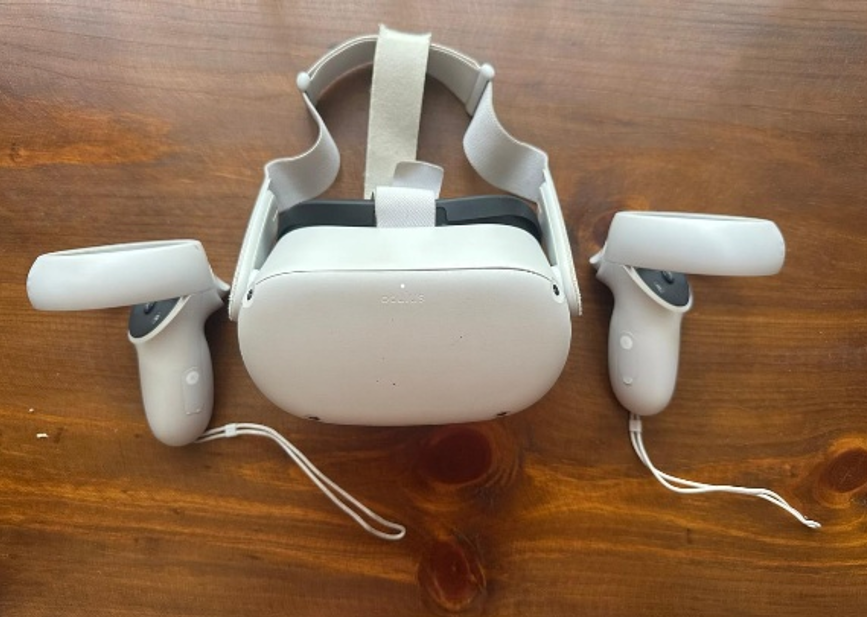
\includegraphics[width=0.65\textwidth]{imagenes/MetaQuest2}
    \caption{Visor Meta Quest 2}
    \label{fig:quest2}
\end{figure}

Para facilitar el desarrollo de aplicaciones para los dispositivos Quest, 
Meta proporciona diferentes paquetes y herramientas que conforman su 
entorno Meta XR. Dentro de Unity, Meta XR Core SDK proporciona 
funcionalidades fundamentales para el desarrollo de aplicaciones 
inmersivas y componentes específicos de la plataforma \cite{metaquestunity}.
Meta, además, proporciona además un rig XR que relaciona la 
representación de la cabeza y los dispositivos de entrada físicos con 
cámaras y elementos virtuales dentro de la escena.

En este proyecto, el Meta Quest 2 es el dispositivo utilizado para 
ejecutar y probar la experiencia en VR. Los mecanismos de entrada 
proporcionadas por el ecosistema Meta permiten obtener información de 
posición, orientación y acciones realizadas por el usuario que, 
posteriormente, puede ser interpretada por los sistemas de interacción 
implementados en Unity. De esta forma, la plataforma Meta proporciona 
la conexión entre las acciones físicas del jugador y los eventos 
utilizados por las mecánicas del videojuego.

% Metodología
\chapter{Metodología}
El desarrollo del proyecto se realizó mediante un proceso por etapas 
orientado a la construcción de un prototipo funcional de videoclip 
gamificado en realidad virtual (VR, por sus siglas en inglés). La 
primera etapa del fue la de la preparación del entorno de desarrollo y la 
implementación de las mecánicas básicas de los minijuegos. Posteriormente 
se incorporaron los mecanismos de interacción en VR, el registro de 
métricas de desempeño, el modelado de estados del jugador y el sistema 
de ajuste dinámico de dificultad (DDA, por sus siglas en inglés). 
Finalmente, los distintos módulos se integraron con el flujo general de 
la experiencia y se realizaron pruebas orientadas a comprobar su 
funcionamiento conjunto.

\section{Enfoque general del desarrollo}
El proyecto se abordó como el desarrollo de un prototipo interactivo en 
tiempo real. Para ello, el sistema se dividió en componentes responsables 
de tareas específicas. Las tareas fueron: interacción en VR, lógica de 
los minijuegos, captura de métricas, representación del estado del 
jugador, adaptación dinámica y comunicación con el flujo global de la 
experiencia. Esta separación permitió desarrollar y validar cada 
componente antes de integrarlo con los demás. 

El sistema de interacción generó los eventos correspondientes a las 
acciones realizadas por el usuario. Dichos eventos alimentaron el 
sistema de métricas, y las métricas registradas se utilizaron para 
determinar el comportamiento del sistema adaptativo. De esta manera, se 
estableció un flujo general de interacción medición, interpretación y 
adaptación. 

La adaptación se diseño utilizando un enfoque basado en reglas. Esta 
decisión permitió relacionar de manera explícita las variables 
observadas durante el gameplay con los cambios realizados sobre los 
minijuegos, facilitando la inspección y ajuste de las condiciones 
utilizadas por el sistema. Así se construyo el modelo sin que fuera un 
modelo clínico o psicológico del usuario, sino una representación 
operativa de su comportamiento basado en información generada 
directamente durante la ejecución.

\section{Preparación del entono de desarrollo en VR}
Lo primero fue configurar el proyecto en Unity para soportar interacción 
XR y se habilitaron los componentes necesarios para reconocer la 
posición y orientación del visor Meta Quest y los dispositivos de 
entrada. Luego, se configuró la representación del usuario dentro de las 
escenas de manera que los movimientos realizados con el dispositivo 
pudieran trasladarse al entorno virtual. A partir de esta configuración 
se comprobó el funcionamiento de la cámara, los controles y las 
interacciones básicas antes de incorporar las mecánicas específicas de 
los minijuegos. 

También se estableció una estructura común para los elementos que 
posteriormente serían utilizados por los distintos sistemas. El objetivo 
fue evitar que cada minijuego tuviera que implementar de forma 
independiente mecanismos equivalentes de entrada, detección o 
comunicación.

Los recursos tridimensionales necesarios para los minijuegos se 
obtuvieron, principalmente, de la \textit{Asset Store} de Unity, pero 
recursos específicos como el modelo de los músicos fueron creados 
utilizando Blender. Todos los modelos siguen una misma dirección visual 
estilizada y un estilo \textit{low-poly}, procurando mantener una 
complejidad adecuada para la ejecución de la experiencia en el Meta 
Quest 2. Una vez preparados o recolectados, los recursos fueron 
importados a Unity y configurados con los componentes necesarios para 
permitir su utilización dentro de las escenas.

\section{Diseño e implementación de los minijuegos}
Se desarrollaron tres minijuegos para representar diferentes formas de 
interacción dentro del videoclip gamificado. Cada uno fue diseñado 
alrededor de una actividad breve que pudiera realizarse utilizando 
acciones físicas dentro del entorno virtual y que permitiera generar 
eventos cuantificables para el sistema adaptativo.

Antes de implementar cada minijuego se definieron sus objetivos, las 
acciones válidas del jugador, las condiciones de acierto y error y los 
elementos susceptibles de modificación durante la ejecución. Esta 
definición permitió separar las reglas fundamentales de cada actividad 
de los parámetros que posteriormente podrían alterarse mediante el DDA.

Las mecánicas se implementaron inicialmente sin adaptación dinámica. 
Esta primera versión permitió comprobar que las acciones pudieran 
completarse correctamente y que existiera una respuesta clara ante los 
resultados del jugador. Posteriormente, se incorporaron los puntos de 
medición necesarios para registrar el desempeño y los parámetros que 
podían ser modificados por el sistema adaptativo.

Aunque cada minijuego utilizó mecánicas diferentes, se mantuvo una 
estructura común para comunicar eventos de interacción y desempeño. Esto 
permitió que el sistema de métricas y adaptación operara sobre 
información equivalente sin depender directamente de la lógica interna de 
una mecánica específica.

\section{Implementación del sistema base de interacción}
Una vez establecidas las mecánicas principales, se implementó el sistema 
encargado de reconocer y procesar las acciones realizadas por el jugador 
dentro del entorno virtual. Este sistema recibió la información 
proveniente de los dispositivos de entrada y la relacionó con los 
objetos interactivos presentes en cada minijuego. La detección de 
interacción se realizó utilizando los mecanismos de colisión y detección 
disponibles en Unity. 

Los objetos relevantes fueron configurados para identificar eventos como 
contacto, selección, impacto o activación, dependiendo de las necesidades 
de cada mecánica. A partir de estos eventos se ejecutaron las reglas 
correspondientes para determinar si una acción representaba un acierto, 
un error o una interacción que no debía ser contabilizada. También se 
implementaron condiciones específicas para controlar cuándo una acción 
podía ser considerada válida. Esto permitió reducir registros duplicados 
y evitar que contactos involuntarios fueran interpretados como múltiples 
interacciones.

Cada acción relevante generó retroalimentación inmediata para comunicar 
al jugador el resultado de su interacción. Se utilizaron respuestas 
visuales, sonoras y hápticas según las características de cada minijuego. 
Estos mecanismos se integraron con la propia lógica de interacción para 
que la respuesta ocurriera en el momento en que el sistema reconocía el 
evento.

\section{Diseño y registro de métricas de desempeño}
Después de comprobar el funcionamiento de las interacciones, se 
implementó un sistema de telemetría destinado a registrar información del 
desempeño del jugador durante la ejecución. Para ello, se seleccionaron 
como variables principales los aciertos, errores, tiempo de reacción, 
precisión y frecuencia de interacción. Estos datos permitieron analizar 
de manera más objetiva la respuesta del jugador ante las distintas 
actividades y obtener información útil para evaluar el funcionamiento de 
la experiencia. 

Los aciertos y errores se registraron a partir del resultado producido 
por las reglas de cada minijuego. Para evitar los que los valores 
dependieran de la lógica interna de una actividad específica, cada 
minijuego comunicó al sistema de métricas el resultado de las 
interacciones relevantes mediante eventos comunes. El tiempo de reacción 
se calculó utilizando el intervalo entre el momento en que una 
oportunidad de interacción se encontraba disponible para el jugador y el 
instante en que se detectaba una respuesta válida. Esta información 
permitió observar cambios en la rapidez de respuesta durante diferentes 
momentos de la experiencia. 

La precisión se utilizó para representar qué tan correctamente se 
ejecutaban aquellas acciones cuya mecánica permitía evaluar la 
correspondencia entre el movimiento realizado y el objetivo establecido. 
Debido a que los minijuegos utilizaban formas de interacción diferentes, 
esta métrica fue normalizada de acuerdo con las características de cada 
actividad antes de ser utilizada por el sistema de adaptación. La 
frecuencia de interacción se obtuvo a partir de la cantidad de acciones 
relevantes detectadas durante un intervalo de tiempo. Esta variable 
permitió diferenciar períodos de actividad continua de momentos en los 
que el usuario reducía o detenía su participación.

Las métricas se mantuvieron disponibles durante la ejecución de la 
experiencia para que pudieran ser consultadas por los sistemas de estados 
y adaptación. Además de los valores acumulados, se consideraron 
observaciones recientes del comportamiento para evitar que el desempeño 
de los primeros momentos de la experiencia condicionara permanentemente 
las decisiones posteriores. De esta manera, el sistema podía actualizar 
la interpretación del desempeño del jugador conforme avanzaba la sesión 
y respondía a las distintas actividades. Esto permitió que las decisiones 
de adaptación se basaran tanto en la evolución general de los resultados 
como en el comportamiento observado en los momentos más recientes.

\section{Modelado de estados del jugador}
A partir de las métricas registradas se desarrolló una representación 
simplificada del estado de interacción del jugador. Se definieron cuatro 
estados operativos: quieto, interactuando, sobrecargado y transicionando. 
Estos estados no representaron diagnósticos psicológicos, sino categorías 
funcionales para la experiencia que resumían patrones observables durante 
su ejecución.

El estado “quieto” se utilizó cuando el sistema detectaba una reducción 
sostenida de las interacciones esperadas. El estado “interactuando” 
representó una participación regular dentro de los parámetros esperados 
para la actividad. El estado “sobrecargado” se usó cuando la combinación 
de métricas mostraba dificultades persistentes para responder 
adecuadamente a las exigencias actuales del minijuego. Finalmente, el 
estado “transicionando” se utilizó durante períodos en los que el flujo 
de la experiencia cambiaba de una actividad a otra y las métricas no 
debían ser interpretadas utilizando las mismas condiciones de una 
interacción activa.

La clasificación no se realizó a partir de un único evento. Se analizaron 
varias observaciones recientes para reducir la posibilidad de cambiar de 
estado como consecuencia de un error aislado o una pausa breve. Asimismo, 
se establecieron condiciones para controlar las transiciones entre 
estados y evitar cambios continuos cuando las métricas se encontraban 
cerca de un límite. 

El estado obtenido se mantuvo disponible como una entrada adicional para 
el sistema adaptativo, complementando las métricas individuales. De esta 
manera, las decisiones de ajuste podían considerar tanto valores 
concretos de desempeño como tendencia general identificada durante el 
período reciente de interacción. Esto permitía que el sistema no 
reaccionara únicamente a resultados aislados, sino que también tuviera en 
cuenta la evolución del comportamiento del jugador a lo largo del tiempo.

\section{Implementación del DDA}
El sistema DDA se desarrolló después de disponer de interacciones 
estables, métricas registrables y una representación del estado del 
jugador. Su funcionamiento se basó en reglas que relacionaban tendencias 
de desempeño con modificaciones sobre parámetros controlables de cada 
minijuego. Estas reglas permitían adaptar progresivamente la experiencia 
según el rendimiento observado, evitando que la dificultad permaneciera 
fija durante toda la sesión.

Se definieron tres categorías principales de parámetros adaptativos: 
velocidad, cantidad de objetos y complejidad de la tarea. La aplicación 
concreta de cada parámetro dependió de las características del minijuego. 
De esta manera, el sistema adaptativo determinaba la dirección del 
cambio, mientras que cada mecánica establecía como debía materializarse 
dicho ajuste.

Las decisiones no se realizaron después de cada interacción individual. 
El sistema acumuló información durante períodos de observación y evaluó 
tendencias antes de aplicar una modificación. Cuando el desempeño se 
mantenía por debajo de los valores esperados o el jugador permanecía en 
el estado de sobrecarga, se aplicaban ajustes orientados a reducir las 
exigencias de la actividad. Cuando se observaba un desempeño estable y 
sostenido, el sistema podía aumentar gradualmente la exigencia. 

También se definieron situaciones en las que la dificultad debía 
mantenerse. Esto evitó que pequeñas variaciones produjeran modificaciones 
innecesarias. Después de ejecutar un cambio se permitió un período de 
estabilización antes de realizar una nueva evaluación, con el propósito 
de observar el efecto de la modificación y reducir oscilaciones continuas 
entre niveles dificultad. 

Los ajustes se limitaron a rangos previamente definidos para cada 
minijuego. De esta manera, el sistema no podía reducir o aumentar los 
parámetros hasta valores que alteren las reglas fundamentales de la 
actividad o produjeran condiciones incompatibles con la experiencia 
musical. El DDA se mantuvo separado de la implementación específica de 
los minijuegos mediante eventos y parámetros configurables. Esta 
separación permitió utilizar una lógica general de adaptación mientras 
cada actividad conservaba el control sobre la forma en que una 
modificación afectaba su \textit{gameplay}.

\section{Integración del sistema adaptativo con la experiencia global}
Una vez implementados los componentes anteriores, el sistema se integró 
con el flujo general del videoclip gamificado. La integración se realizó 
mediante eventos que permitieron recibir información procedente del 
sistema global y comunicar resultados relacionados con el desempeño del 
jugador. De esta forma, las acciones realizadas durante los minijuegos 
podían influir en el desarrollo de la experiencia y en la actualización 
de las métricas correspondientes.

El sistema adaptativo recibió notificaciones necesarias para conocer el 
contexto general de ejecución, por ejemplo, el inicio o finalización de 
una actividad o el ingreso a un período de transición. Estas señales se 
utilizaron para controlar cuándo debía comenzar o detenerse la captura e 
interpretación de las métricas. De manera inversa, los minijuegos y los 
sistemas de interacción emitieron información relacionada con aciertos, 
errores, progreso y desempeño. Esta comunicación permitió mantener 
desacoplada la lógica adaptativa de los componentes responsables del 
flujo global de la experiencia.

\section{Pruebas de calibración y ajustes}
Las pruebas del sistema adaptativo se realizaron provocando diferentes 
patrones de desempeño para comprobar que las reglas reaccionaran en la 
dirección esperada. Se evaluaron escenarios de desempeño sostenido, 
sucesión de errores, ausencia temporal de interacción y recuperación 
posterior del jugador. Esto permitió observar las transiciones entre 
estados y verificar que los parámetros de dificultad fueran modificados 
únicamente cuando se cumplían las condiciones establecidas.

Posteriormente, se ajustaron los umbrales, períodos de observación, 
límites de los parámetros y tiempos entre modificaciones. Esta 
calibración se hizo para evitar oscilaciones frecuentes entre 
configuraciones de dificultad. Con esto el sistema ya solo aplicaba una 
modificación cuando existían suficientes indicios de que el nivel de 
dificultad debía mantenerse, aumentarse o reducirse. Finalmente, el 
prototipo fue probado como una experiencia integrada utilizando el Meta 
Quest 2 para comprobar la interacción física, la retroalimentación, la 
captura de datos y la respuesta del sistema adaptativo. 






% Resultados

% Análisis y discusión

% Conclusiones

% Bibliografía
\clearpage
\addcontentsline{toc}{chapter}{Bibliografía}
\bibliography{referencias}

% Anexos
\clearpage

\end{document}
